\chapter{Título do Capítulo 2}
\label{cap2}

Este capítulo exemplifica a utilização de referências, figuras, tabelas e listagens.

\section{Titulo de uma seção}
Deve haver aqui uma frase.

\subsection{Título de uma subseção}
\subsubsection{Título de parágrafo de texto normal}

Eis duas citações \cite{book:Brooks1995,Chen1976}.

A Figura \ref{fig:exemplofig} apresenta os vários tipos de diagrama da Unified Modeling Language (UML).

\begin{figure}[!htb]
\centering
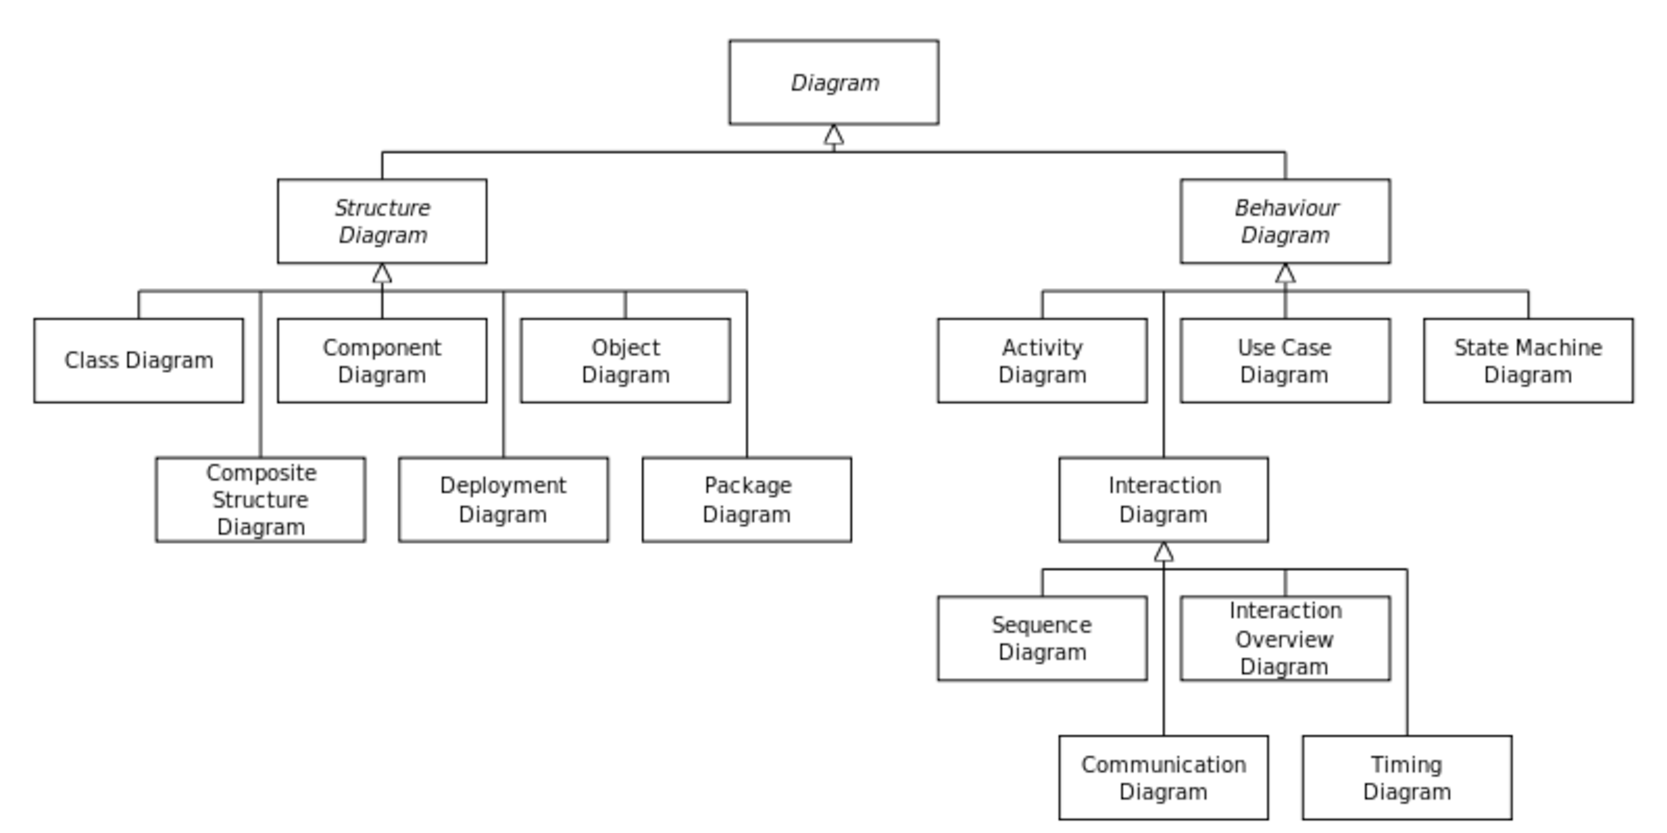
\includegraphics[width=16cm]{exemploFig}
\caption{Exemplo de Figura (\textit{in} \url{http://en.wikipedia.org/wiki/Class_diagram})}
\label{fig:exemplofig}
\end{figure}

Exemplos de citações \cite{AndroidDoc},
\cite{Huetal2000,book:Brooks1995,Chen1976}

%Exemplo de listagem de código Java.
%\lstlisting{

\section{Exemplos de Listagens}

A Listagem \ref{lst:py} apresenta um exemplo de implementação do algoritmo de ordenação \textit{quicksort} na linguagem de programação Python.

\begin{lstlisting}[language=python,caption={Exemplo de listagem de código Pythonescrito directamente no ficehiro tex (apenas recomendado para 1 a 5 linhas de código},{label=lst:py}]
# in http://www.ics.uci.edu/~eppstein/161/python/quicksort-inplace.py - 2013/04/14
# quick sort, in-place 3-way partition
# David Eppstein, UCI, 17 Jan 2002
def swap(A,i,j):
	temp = A[i]
	A[i] = A[j]
	A[j] = temp
\end{lstlisting}


A Listagem \ref{lst:java} apresenta um exemplo de implementação do algoritmo de ordenação \textit{quicksort} na linguagem de programação \Java{}.

\lstinputlisting[language=java,caption={Exemplo de listagem de código Java importado de um ficheiro na pasta listagens.},{label=lst:java}]{listagens/quicksort.java}

\lstinputlisting[language=java,caption={Exemplo de listagem de parte de um ficheiro Java na pasta listagens.},{label=lst:javaparcial},firstline=38,lastline=44]{listagens/quicksort.java}


\pagebreak % para forçar uma mudança de página
%%%%%%%%%%%%%%%%%%%%
\section{Um exemplo de tabela}

A Tabela \ref{tab:caso} apresenta os resultados de aplicação de quatro métodos a um caso.

%baseado num exemplo em http://www1.maths.leeds.ac.uk/latex/TableHelp1.pdf
\begin{table}[htb]
\caption{Uma tabela de exemplo} % título da tabela
\centering % para centrar a tabela
\begin{tabular}{l l c r} % duas colunas à esquerda (l l), uma ao centro (c) e uma à direita (r) (4 colunas)
\hline\hline %insere duas linhas horizontais
Caso & Método 1 & Método 2 & Método 3 \\ [0.5ex] % insere tabela 
\hline % insere uma linha horizontal
1 & 50 & 837 & 970 \\ % insure corpo da tabela
2 & 47 & 877 & 230 \\
3 & 31 & 25 & 415 \\
4 & 35 & 144 & 2356 \\
5 & 45 & 300 & 556 \\ [1ex] % [1ex] adiciona espaço vertical
\hline %insere uma linha horizontal
\end{tabular}
\label{tab:caso} % é utilizada para referir a tabela no texto
\end{table}




